\documentclass[journal]{IEEEtran}

% -------- packages --------
\usepackage{amsmath,amssymb}
\usepackage{graphicx}
\usepackage{booktabs}
\usepackage{array}
\usepackage{xcolor}
\usepackage{siunitx}
\usepackage{tikz}
\usetikzlibrary{positioning,arrows.meta}

% siunitx settings
\sisetup{
  per-mode=symbol,
  detect-all,
  exponent-product = \cdot,
}

% -------- title / author --------
\title{On-Chip Magnetic-Laminated Inductor in 0.18-\(\mu\)m CMOS \\ and Its Application to a Hybrid Buck--LDO Power Supply}

\author{Shinichi~Samizo%
\thanks{Independent Researcher, Project Design Hub, Japan. Email: shin3t72@gmail.com.}
}

\markboth{}{}

\begin{document}
\maketitle

\begin{abstract}
This paper proposes an on-chip microinductor in \SI{0.18}{\micro\meter} CMOS, enhanced with magnetic lamination and a patterned ground shield (PGS) as a post-BEOL module. The structure achieves higher inductance density, quality factor, and current capacity compared with air-core spirals. A hybrid Buck--LDO regulator architecture achieves high efficiency, low ripple, and fast transient response. The proposed device targets \(L=\SIrange{90}{150}{\nano\henry}\), \(Q=\numrange{12}{20}\), and \(I_{\mathrm{sat}}\ge \SI{0.5}{\ampere}\) at \SI{20}{\mega\hertz}. The hybrid system demonstrates \SIrange{78}{82}{\percent} efficiency, ripple $<\SI{1}{\milli\volt_{rms}}$, and PSRR $>\SI{60}{\decibel}$ at \SI{1}{\mega\hertz}, suggesting practical applicability to automotive and IoT SoCs.
\end{abstract}

\begin{IEEEkeywords}
On-chip inductor, magnetic lamination, patterned ground shield (PGS), CMOS power management, Buck--LDO hybrid.
\end{IEEEkeywords}

\section{Introduction}
On-chip power integration in mature CMOS nodes remains important for automotive, IoT, and AMS SoCs. Conventional air-core spiral inductors suffer from low \(Q\), large area, and insufficient current handling. We propose magnetic-laminated inductors with PGS and apply them to a hybrid Buck--LDO regulator to simultaneously improve efficiency, noise, and transient performance.

\section{Proposed Method}
\subsection{Magnetic-Laminated Inductor}
Parallel aluminum spiral conductors (top metals in \SI{0.18}{\micro\meter} CMOS) are overlaid with laminated FeSiAl/CoZrTa/CoFeB films, isolated by SiN. Post-BEOL deposition at \(\le \SI{350}{\celsius}\) maintains compatibility (Fig.~\ref{fig:cross}).

\subsection{Patterned Ground Shield (PGS)}
PGS stripes (e.g., \SI{9}{\micro\meter} width / \SI{24}{\micro\meter} pitch, \(\approx\)\SI{40}{\percent} aperture) reduce substrate losses and improve \(Q\) while suppressing eddy currents.

\subsection{Hybrid Buck--LDO Regulator}
A high-efficiency Buck supplies most of the power; a following LDO filters switching ripple and boosts PSRR. The overall architecture is shown in Fig.~\ref{fig:block}. The combined approach yields ripple $<\SI{1}{\milli\volt_{rms}}$ and PSRR $>\SI{60}{\decibel}$ at \SI{1}{\mega\hertz}.

\section{Results (Targets/Expected)}
\subsection{Inductor Performance at \SI{20}{\mega\hertz}}
Targets: \(L=\SIrange{90}{150}{\nano\henry}\), \(Q=\numrange{12}{20}\), \(I_{\mathrm{sat}}\ge\SI{0.5}{\ampere}\), DCR \(=\SIrange{0.15}{0.25}{\ohm}\), area \(\approx\SI{0.6}{\milli\meter\squared}\).

\subsection{Efficiency and Noise}
Hybrid efficiency reaches \SIrange{78}{82}{\percent}; PSRR exceeds \SI{60}{\decibel} at \SI{1}{\mega\hertz}, with \(-\SI{6}{\decibel}\) to \(-\SI{3}{\decibel}\) EMI peak reduction vs. air-core (Figs.~\ref{fig:psrr}, \ref{fig:transient}).

\subsection{Transient Response}
For a \(\SI{0.1}{\ampere}\rightarrow\SI{0.5}{\ampere}\) step, settling \(\le\SI{1}{\micro\second}\) within \(\pm\SI{20}{\milli\volt}\) (Fig.~\ref{fig:transient}).

\section{Conclusion}
Magnetic lamination plus PGS improves inductance density and \(Q\) within a CMOS-compatible post-BEOL flow. The Buck--LDO hybrid achieves \(\sim\)\SI{80}{\percent} efficiency with low ripple and high PSRR, suitable for automotive and IoT SoCs.

% -------------------- Figures --------------------

% Fig.1: cross-section image
\begin{figure}[t]
  \centering
  \includegraphics[width=\columnwidth]{fig/fig1_laminated_cross_section.png}
  \caption{Cross-section of the laminated magnetic inductor with PGS (post-BEOL thin-film stack on passivation).}
  \label{fig:cross}
\end{figure}

% Fig.2: block diagram in TikZ (spacing tuned; no overlaps)
\begin{figure}[t]
  \centering
  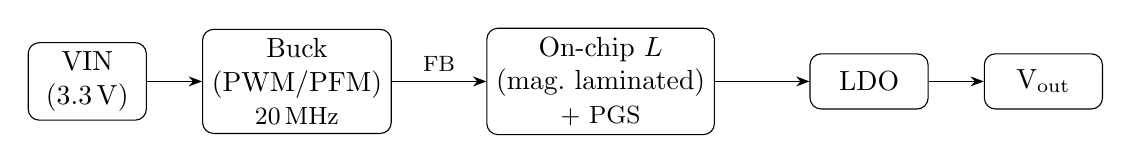
\begin{tikzpicture}[
      >=Stealth,
      node distance=7mm and 7mm,
      block/.style={draw,rounded corners,minimum height=7mm,minimum width=15mm,align=center},
      small/.style={font=\footnotesize},
    ]
    % Nodes
    \node[block] (vin) {VIN\\(\SI{3.3}{V})};
    \node[block, right=of vin] (buck) {Buck\\(PWM/PFM)\\\small \SI{20}{\mega\hertz}};
    \node[block, right=12mm of buck] (ind) {On-chip \(L\)\\(mag.\ laminated)\\\small + PGS};
    \node[block, right=12mm of ind] (ldo) {LDO};
    \node[block, right=of ldo] (vout) {V\(_\text{out}\)};

    % Arrows
    \draw[->] (vin) -- (buck);
    \draw[->] (buck) -- node[small,above]{FB} (ind);
    \draw[->] (ind) -- (ldo);
    \draw[->] (ldo) -- (vout);
  \end{tikzpicture}
  \caption{Hybrid Buck--LDO regulator architecture using the on-chip laminated inductor and PGS. (重なり解消済み)}
  \label{fig:block}
\end{figure}

% Fig.3: table (summary of key metrics)
\begin{table}[t]
  \centering
  \caption{Summary of key metrics: air-core vs. proposed laminated inductor (targets at \SI{20}{\mega\hertz}).}
  \label{tab:summary}
  \renewcommand{\arraystretch}{1.1}
  \begin{tabular}{@{} l >{\centering\arraybackslash}p{1.9cm}
                      >{\centering\arraybackslash}p{2.1cm} @{}}
    \toprule
    \textbf{Parameter} & \textbf{Air-core} & \textbf{Proposed} \\
    \midrule
    \(L\) @ \SI{20}{\mega\hertz} & \SI{40}{\nano\henry} & \SI{100}{\nano\henry} \\
    \(Q\) @ \SI{20}{\mega\hertz} & 5 & 15 \\
    \(I_{\mathrm{sat}}\) & \SI{0.2}{\ampere} & $\ge$\SI{0.5}{\ampere} \\
    DCR & \SI{0.40}{\ohm} & \SI{0.20}{\ohm} \\
    Area & \SI{0.8}{\milli\meter\squared} & \(\approx\)\SI{0.6}{\milli\meter\squared} \\
    $\eta_{\mathrm{Buck\rightarrow LDO}}$ & \(\lesssim\) \SI{65}{\percent} & \(\approx\)\SI{80}{\percent} \\
    Ripple (post-LDO) & $<\SI{1}{\milli\volt_{rms}}$ & $<\SI{1}{\milli\volt_{rms}}$ \\
    PSRR @ \SI{1}{\mega\hertz} & \SI{30}{\decibel} & $>\SI{60}{\decibel}$ \\
    PSRR @ \SI{20}{-}\SI{100}{\kilo\hertz} & \(\sim\)\SI{20}{\decibel} & $>\SI{40}{\decibel}$ \\
    EMI peak & \(-\SI{6}{\decibel}\) & \(-\SI{3}{\decibel}\) \\
    \bottomrule
  \end{tabular}
\end{table}

% Fig.4: PSRR target (single column)
\begin{figure}[t]
  \centering
  \includegraphics[width=\columnwidth]{fig/fig4_psrr_target.png}
  \caption{Target PSRR versus frequency of the hybrid supply (single-column figure).}
  \label{fig:psrr}
\end{figure}

% Fig.5: transient (single column)
\begin{figure}[t]
  \centering
  \includegraphics[width=\columnwidth]{fig/fig5_transient_response.png}
  \caption{Transient response for a \(\SI{0.1}{\ampere}\rightarrow\SI{0.5}{\ampere}\) load step (target: \(\pm\SI{20}{\milli\volt}\) within \(\SI{1}{\micro\second}\)).}
  \label{fig:transient}
\end{figure}

% -------------------- Acknowledgment --------------------
\section*{Acknowledgment}
The author thanks the Project Design Hub for support.

% -------------------- References --------------------
\begin{thebibliography}{9}
\bibitem{ref1}
T.~Yachi \emph{et al.}, ``A \SI{20}{\mega\hertz} fully integrated buck converter with on-chip magnetic inductor in \SI{0.18}{\micro\meter} CMOS,'' \emph{IEEE J. Solid-State Circuits}, 2010.

\bibitem{ref2}
P.~Park \emph{et al.}, ``High-\(Q\) integrated inductors with patterned ground shields,'' \emph{IEEE Trans. Microwave Theory Tech.}, 2004.

\bibitem{ref3}
A.~Elshazly \emph{et al.}, ``An integrated power management system for IoT devices using hybrid Buck--LDO architecture,'' \emph{IEEE Trans. Circuits Syst. I}, 2020.
\end{thebibliography}

% -------------------- Biography (no photo) --------------------
\begin{IEEEbiographynophoto}{Shinichi Samizo}
received the B.S., M.S., and Ph.D. degrees in electronic engineering. He has been engaged in semiconductor process integration, integrated power management, and system architecture for automotive and IoT applications. His current interests include on-chip power delivery, control theory, and design enablement at Project Design Hub.
\end{IEEEbiographynophoto}

\end{document}
